\documentclass[twocolumn, a4paper]{article}
\usepackage[a4paper, left = 1.75cm, right = 1.75cm, top = 1.75cm, bottom = 1.75cm]{geometry}
\usepackage[style = numeric, sorting = none]{biblatex}
\usepackage{pgfplots}
\usepackage[T1]{fontenc}
\usepackage{graphicx}
\usepackage{arydshln}
\usepackage[UKenglish]{babel}
\usepackage[UKenglish]{isodate}

\graphicspath{{./images/}}
\addbibresource{refs.bib}

\cleanlookdateon

\renewcommand*{\bibfont}{\footnotesize}

\author{
  George Herbert\\
  \texttt{cj19328@bristol.ac.uk}
}

\title{Parallelising the Lattice Boltzmann Method}

\begin{document}

\maketitle

\begin{abstract}
  The Lattice Boltzmann method (LBM) simulates a fluid density on a lattice.
  This report analyses the techniques I utilised to produce three implementations of LBM: one with distributed-memory parallelism, using Message Passing Interface (MPI) for interprocess communication; one hybrid, using a combination of MPI and OpenMP; the third used OpenCL to run on a GPU.
\end{abstract}

\section{Single Program, Multiple Data}

\subsection{Hypothesis}

My OpenMP implementation of \texttt{d2q9-bgk.c} with shared-memory parallelism achieved a substantial speedup over my serial implementation.
However, it was limited to a single node of BC4, which was a considerable restriction.

Single program, multiple data (SPMD) is a form of parallelism in which independent processes run the same program.
Message Passing Interface (MPI) is a specification for a library interface for passing messages between processes.
Therefore, I hypothesised that implementing of \texttt{d2q9-bgk.c} with distributed memory parallelism that ran on multiple processes across multiple nodes---with MPI used for interprocess communication---would provide an even more significant speedup.

\subsection{Compiler}

I used the \texttt{mpiicc} wrapper script, which compiled my program with the Intel C Compiler Classic (version 19.1.3.304) and set up the include and library paths for the Intel MPI library.
I compiled my program with the \texttt{-std=c99}, \texttt{-Wall}, \texttt{-Ofast}, \texttt{-restrict} and \texttt{-xAVX2} options.

\subsection{Load Balancing}

I had to assign different sections of the grid to different processes explicitly.
The distribution needed to be adequately balanced to minimise the time processes' spent blocked.

Since the \texttt{cells} grid was in row-major order, I split the grid horizontally between processes to take advantage of memory locality.
I created a procedure \texttt{allocate\_rows} to balance the load.
The procedure assigned each process at least $\lfloor\frac{y}{n}\rfloor$ consecutive rows, with the first $y - \lfloor\frac{y}{n}\rfloor n$ processes each assigned an additional consecutive row, where $y$ was the number of rows and $n$ the number of processes.
Additionally, since updating the value of a given cell required the values of all adjacent cells, each process contained two additional rows reserved for cells in the top and bottom rows of the preceding and succeeding ranks, respectively.
Figure \ref{fig:rows} displays an example allocation for a grid with five rows split between two processes; the green rows are those allocated to the process, whilst the red rows are the additional rows required to update the edge rows correctly.

\begin{figure}[htbp]
  \centering
  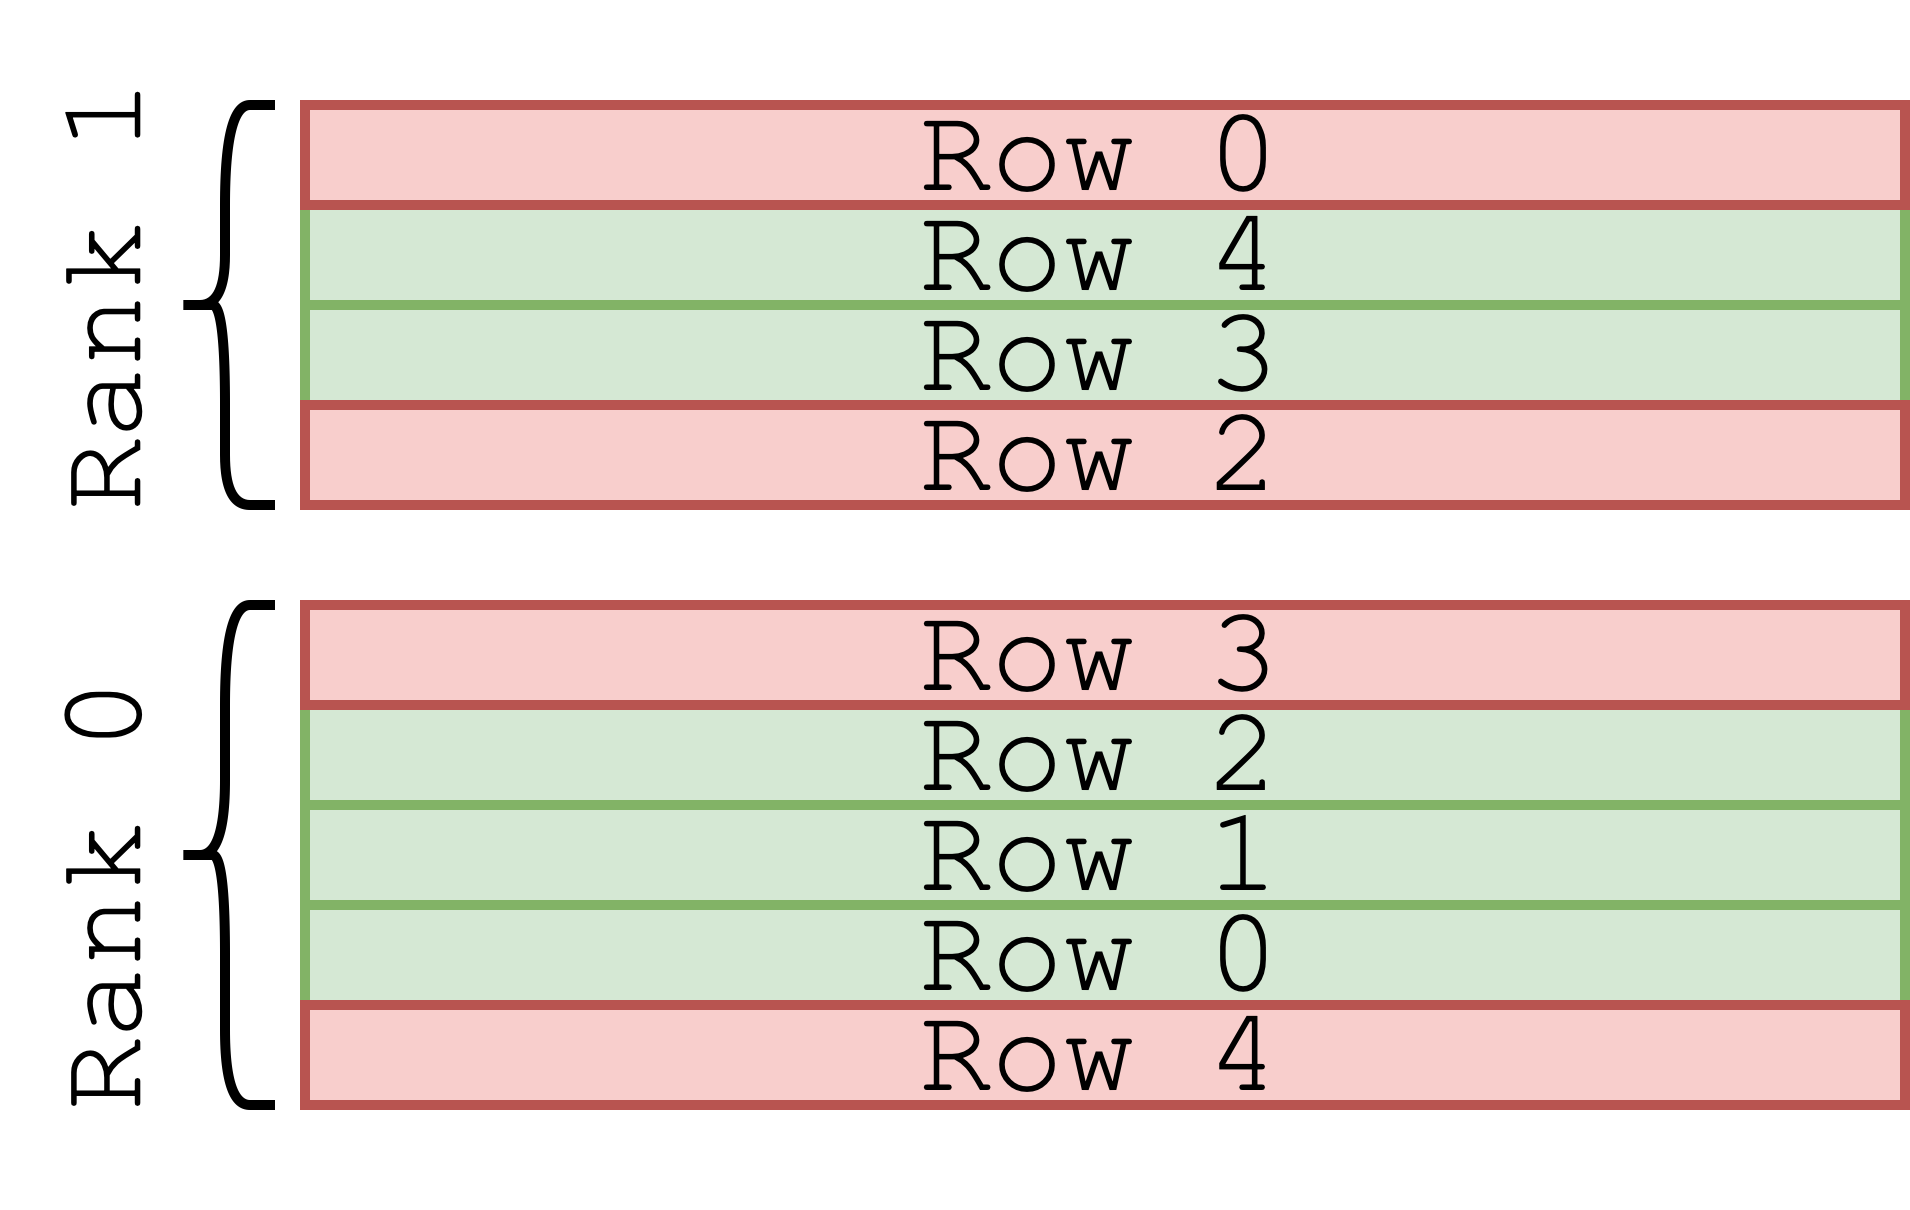
\includegraphics[width=.75\linewidth]{rows.png}
  \caption{Row allocation example with five rows and two processes}\label{fig:rows}
\end{figure}

I decided against splitting on a sub-row level to avoid unnecessarily increasing the complexity of my program and incurring additional computational overhead.

\subsection{Halo Exchange}

Since processes are assigned an individual virtual memory region, I had to explicitly send the contents of edge rows to neighbouring ranks after each timestep.
To do so, I created a \texttt{halo\_exchange} procedure.
The procedure copied the bottom-most row allocated to the process into the \texttt{send\_row\_buffer} array.
Since the \texttt{cells} data was in the structure of arrays (SoA) format, the values from the nine separate arrays of speeds had to be packed into the buffer.
I used the \texttt{MPI\_Sendrecv} procedure to send this buffer to the \texttt{receive\_row\_buffer} of the preceding rank.
Then, the procedure copied the values into the additional upper row---unpacking the values into the nine separate arrays of speeds.
The same process was then repeated for the top-most row, which was sent to the succeeding rank.

\subsection{Collating}

I created a \texttt{collate} procedure that was executed once all iterations of the \texttt{timestep} procedure were complete.
The procedure had two purposes.
The first purpose was to transfer the final state of the cells allocated to each process to the master process (i.e. rank zero).
The second purpose was to transfer the partial average velocity values to the master process and use these values to calculate the correct average velocity at each timestep.

I used the \texttt{MPI\_Send} procedure to send the final state of the cells allocated to each process to the master process.
The master process received these values by executing the \texttt{MPI\_Recv} procedure once for each process.

I also used the \texttt{MPI\_Send} procedure to send each process' partial average velocity values to the master process.
The master process received these arrays of values consecutively from each process using the \texttt{MPI\_Recv} procedure and summed them into a global average velocities array.
The \texttt{collate} procedure then multiplied each element by \texttt{params.num\_non\_obstacles\_r} in the master process to calculate the correct average velocity at each timestep.

\subsection{Results}

Table \ref{tab:mpi} displays the results of my MPI implementation.
Each time was an average of three runs on BlueCrystal Phase 4 (BC4) compute nodes, which were each a Lenovo nx360 M5, which contained two 14-core 2.4 GHz Intel E5-2680 v4 (Broadwell) CPUs and 128 GiB of RAM \cite{bcp4}.
My MPI implementation provided a substantial speedup over both my serial optimised implementation and my OpenMP implementation.
My program achieved the speedup by executing sections of the \texttt{timestep} procedure in parallel, utilising 112 times more L1 and L2 cache and utilising eight times more L3 cache.

\begin{table}[htbp]
  \begin{center}
  \caption{Execution times with the 112 process MPI implementation and speedup over both my serial optimised and 28 thread OpenMP implementation}\label{tab:mpi}
  \begin{tabular}[t]{l | l  l  l} 
      \hline\hline
      &&\multicolumn{2}{c}{Speedup}\\
      \cline{3-4}
      Grid Size&Time (s)&Serial&OpenMP\\
      \hline
      $128 \times 128$&\texttt{}&\texttt{}&\texttt{}\\
      $128 \times 256$&\texttt{}&\texttt{}&\texttt{}\\
      $256 \times 256$&\texttt{}&\texttt{}&\texttt{}\\
      $1024 \times 1024$&\texttt{}&\texttt{}&\texttt{}\\
      \hline
    \end{tabular}
  \end{center}
\end{table}

\section{Optimisations}

\subsection{Average Velocities Reduction}

I hypothesised I could use the \texttt{MPI\_Reduce} procedure to speed up the collation time of my program.
Table \ref{tab:reduction} contains the collation times for this implementation and speedup over the prior implementation.
Using \texttt{MPI\_Reduce} led to a significant reduction in collation time.
However, this did not significantly affect the overall execution time because the collation time was short compared to the compute time.
I would expect a more significant impact on the overall execution time for inputs containing more iterations.

\begin{table}[htbp]
  \begin{center}
  \caption{Collate times with the reduction and speedup over the prior implementation}\label{tab:reduction}
  \begin{tabular}[t]{l | l l} 
      \hline\hline
      Grid Size&Time (s)&Speedup\\
      \hline
      $128 \times 128$&\texttt{0.0016}&\texttt{4.54}\\
      $128 \times 256$&\texttt{0.0029}&\texttt{2.93}\\
      $256 \times 256$&\texttt{0.0049}&\texttt{2.83}\\
      $1024 \times 1024$&\texttt{0.0420}&\texttt{1.08}\\
      \hline
    \end{tabular}
  \end{center}
\end{table}

\section{Analysis}

\subsection{Scaling}

I ran my final MPI implementation from 1--112 processes to analyse how my program scaled.
My program ran on as few nodes as possible, with each process assigned to a single core. 
I then calculated the subsequent processes' speedup over a single process implementation.
Figure \ref{fig:scaling} displays the result speedup curves.

\begin{figure}[htpb]
  \centering
  \resizebox{\columnwidth}{!}{
    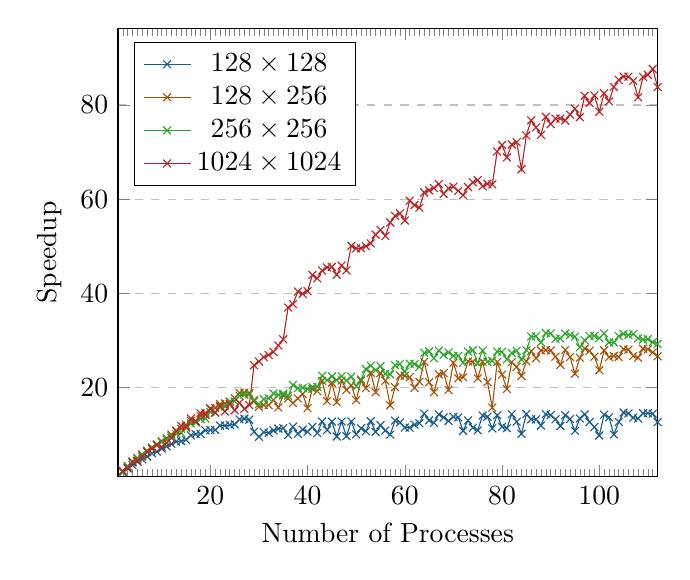
\begin{tikzpicture}
      \begin{axis}[
        xlabel={Number of Processes},
        ylabel={Speedup},
        xmin = 1, xmax = 112,
        ymin = 1,
        % xtick={0, 5, 10, 15, 20, 25},
        % ytick={0,20,40,60,80,100,120},
        legend pos=north west,
        ymajorgrids=true,
        grid style=dashed,
        minor xtick = {1, 2, 3, 4, 5, 6, 7, 8, 9, 10, 11, 12, 13, 14, 15, 16, 17, 18, 19, 20, 21, 22, 23, 24, 25, 26, 27, 28, 29, 30, 31, 32, 33, 34, 35, 36, 37, 38, 39, 40, 41, 42, 43, 44, 45, 46, 47, 48, 49, 50, 51, 52, 53, 54, 55, 56, 57, 58, 59, 60, 61, 62, 63, 64, 65, 66, 67, 68, 69, 70, 71, 72, 73, 74, 75, 76, 77, 78, 79, 80, 81, 82, 83, 84, 85, 86, 87, 88, 89, 90, 91, 92, 93, 94, 95, 96, 97, 98, 99, 100, 101, 102, 103, 104, 105, 106, 107, 108, 109, 110, 111, 112}
      ]
      \addlegendentry{$128\times128$}
      \addplot[color = {rgb:red,31;green,119;blue,180}, mark = x]coordinates{
        (1)
        (2, 1.923484904)
        (3, 2.720894881)
        (4, 3.440629879)
        (5, 4.138267014)
        (6, 4.663357796)
        (7, 5.242110909)
        (8, 5.997834661)
        (9, 6.289791841)
        (10, 6.946565607)
        (11, 7.428037519)
        (12, 7.95038628)
        (13, 8.433876381)
        (14, 8.529248058)
        (15, 8.803834029)
        (16, 9.766209845)
        (17, 10.03121078)
        (18, 10.06840901)
        (19, 10.823501)
        (20, 10.89601518)
        (21, 10.91800443)
        (22, 11.84262736)
        (23, 11.8219416)
        (24, 11.97369741)
        (25, 12.0975617)
        (26, 13.1584053)
        (27, 13.31030358)
        (28, 13.09199604)
        (29, 10.51279543)
        (30, 9.447423254)
        (31, 10.42385535)
        (32, 10.30054902)
        (33, 10.80235067)
        (34, 11.18228843)
        (35, 11.28177199)
        (36, 9.84586148)
        (37, 11.58823901)
        (38, 10.08001059)
        (39, 10.99390174)
        (40, 10.5569982)
        (41, 11.56726497)
        (42, 10.24545739)
        (43, 12.72036597)
        (44, 10.89204809)
        (45, 12.68270324)
        (46, 9.517212061)
        (47, 12.70287876)
        (48, 9.582852227)
        (49, 12.70536401)
        (50, 9.965823544)
        (51, 11.25846097)
        (52, 10.63104034)
        (53, 12.76248403)
        (54, 10.50652785)
        (55, 11.90630364)
        (56, 10.76817156)
        (57, 9.92607211)
        (58, 12.89249626)
        (59, 12.51463609)
        (60, 11.41730712)
        (61, 11.38075986)
        (62, 12.05183804)
        (63, 12.33484451)
        (64, 14.36825721)
        (65, 12.94409609)
        (66, 12.41719085)
        (67, 14.19480666)
        (68, 13.57486626)
        (69, 12.82320169)
        (70, 13.70570713)
        (71, 13.56967231)
        (72, 10.71067935)
        (73, 12.95178741)
        (74, 11.37959467)
        (75, 10.82015609)
        (76, 13.97900377)
        (77, 13.7270023)
        (78, 11.23829384)
        (79, 14.05923951)
        (80, 11.55316639)
        (81, 11.2926889)
        (82, 14.27943961)
        (83, 12.66856962)
        (84, 10.09500034)
        (85, 14.28261536)
        (86, 13.16863695)
        (87, 13.18328092)
        (88, 11.84068965)
        (89, 14.27750429)
        (90, 14.05330958)
        (91, 13.16981575)
        (92, 11.72223637)
        (93, 14.04375416)
        (94, 13.24823774)
        (95, 10.70439261)
        (96, 13.35667621)
        (97, 14.2305021)
        (98, 12.59951023)
        (99, 11.54477978)
        (100, 9.726436232)
        (101, 14.16020099)
        (102, 13.58441421)
        (103, 9.940775763)
        (104, 12.61740837)
        (105, 14.60476445)
        (106, 14.41749489)
        (107, 13.5330826)
        (108, 13.33602024)
        (109, 14.45781616)
        (110, 14.46196727)
        (111, 14.37893291)
        (112, 12.55231676)
      };
      \addlegendentry{$128\times256$}
      \addplot[color = {rgb:red,255;green,127;blue,14}, mark = x]coordinates{
        (1)
        (2, 2.205625975)
        (3, 3.227329026)
        (4, 4.206536128)
        (5, 4.957628857)
        (6, 5.720325252)
        (7, 6.5186293)
        (8, 7.204187632)
        (9, 7.83187371)
        (10, 8.519480837)
        (11, 9.141792188)
        (12, 9.946144856)
        (13, 10.78303952)
        (14, 11.17654785)
        (15, 11.96372797)
        (16, 12.86100085)
        (17, 12.77900855)
        (18, 13.84474552)
        (19, 14.54722804)
        (20, 15.51467595)
        (21, 15.61471426)
        (22, 16.41110324)
        (23, 16.55474236)
        (24, 16.88471919)
        (25, 17.63506903)
        (26, 18.81278116)
        (27, 18.85990554)
        (28, 18.79353144)
        (29, 16.99774639)
        (30, 15.79817866)
        (31, 16.19702524)
        (32, 16.15965593)
        (33, 17.29162535)
        (34, 15.70016114)
        (35, 18.24326824)
        (36, 17.59400273)
        (37, 16.60271485)
        (38, 17.62056876)
        (39, 18.54799616)
        (40, 15.55440163)
        (41, 19.67959722)
        (42, 19.1560423)
        (43, 21.35522276)
        (44, 17.03686616)
        (45, 20.92098931)
        (46, 16.81730667)
        (47, 21.42591543)
        (48, 19.41596955)
        (49, 20.40834137)
        (50, 17.25017866)
        (51, 21.42281112)
        (52, 19.78933109)
        (53, 23.07737542)
        (54, 18.918754)
        (55, 23.01384332)
        (56, 21.37017128)
        (57, 16.14969542)
        (58, 20.0009934)
        (59, 22.46020712)
        (60, 22.42917414)
        (61, 22.12510191)
        (62, 19.87277518)
        (63, 21.15162638)
        (64, 25.37114287)
        (65, 21.04839449)
        (66, 18.95802252)
        (67, 22.70932312)
        (68, 22.97178595)
        (69, 19.42403684)
        (70, 25.20246959)
        (71, 21.87162616)
        (72, 22.10931871)
        (73, 25.48457214)
        (74, 25.40576875)
        (75, 21.86621052)
        (76, 25.42855553)
        (77, 21.08392509)
        (78, 15.6640675)
        (79, 25.37761189)
        (80, 22.68812171)
        (81, 19.62011193)
        (82, 25.34038719)
        (83, 24.32976857)
        (84, 22.38365252)
        (85, 25.49728852)
        (86, 27.67149109)
        (87, 26.16157312)
        (88, 27.82572378)
        (89, 27.90751086)
        (90, 27.82654636)
        (91, 26.48489496)
        (92, 24.75372864)
        (93, 27.9508939)
        (94, 26.41014954)
        (95, 22.85484751)
        (96, 26.26628274)
        (97, 28.21556741)
        (98, 27.73270133)
        (99, 26.49618844)
        (100, 23.61317402)
        (101, 27.82729043)
        (102, 26.40723599)
        (103, 26.65524278)
        (104, 26.4087459)
        (105, 28.08446357)
        (106, 27.97894075)
        (107, 26.65102998)
        (108, 26.26789063)
        (109, 28.17805085)
        (110, 28.07259611)
        (111, 27.39171519)
        (112, 26.56061497)
      };
      \addlegendentry{$256\times256$}
      \addplot[color = {rgb:red,44;green,160;blue,44}, mark = x]coordinates{
        (1)
        (2, 1.925127415)
        (3, 3.140333019)
        (4, 4.034925801)
        (5, 4.78762859)
        (6, 5.548938663)
        (7, 6.404618662)
        (8, 6.968739974)
        (9, 7.663080488)
        (10, 8.312526115)
        (11, 8.852461517)
        (12, 9.605431059)
        (13, 10.06145238)
        (14, 10.29374937)
        (15, 11.37306684)
        (16, 12.28185633)
        (17, 12.50338781)
        (18, 13.18889042)
        (19, 13.31294585)
        (20, 14.70777733)
        (21, 14.55264271)
        (22, 15.75611214)
        (23, 15.92868238)
        (24, 16.95789156)
        (25, 17.02232096)
        (26, 18.1996368)
        (27, 18.42801124)
        (28, 18.46672465)
        (29, 17.29202644)
        (30, 16.3773773)
        (31, 17.47308485)
        (32, 17.62638401)
        (33, 18.65075869)
        (34, 18.39755995)
        (35, 18.60686115)
        (36, 18.19979983)
        (37, 20.47095888)
        (38, 19.78039772)
        (39, 19.87870191)
        (40, 19.57366035)
        (41, 20.0423534)
        (42, 20.04684952)
        (43, 22.41860194)
        (44, 21.51447621)
        (45, 22.29960449)
        (46, 21.51985585)
        (47, 22.32706386)
        (48, 21.42352302)
        (49, 22.23288533)
        (50, 20.21625868)
        (51, 21.66294914)
        (52, 23.84329098)
        (53, 24.58609618)
        (54, 23.59494944)
        (55, 24.47228876)
        (56, 22.8398099)
        (57, 22.7149941)
        (58, 24.69497187)
        (59, 24.92866935)
        (60, 23.2764513)
        (61, 25.00215927)
        (62, 24.92609823)
        (63, 24.28449993)
        (64, 27.31102246)
        (65, 27.61766033)
        (66, 26.16929081)
        (67, 27.76095551)
        (68, 26.85523603)
        (69, 27.40893503)
        (70, 26.66846158)
        (71, 26.67769083)
        (72, 25.19788674)
        (73, 27.57875103)
        (74, 27.87808785)
        (75, 25.09623612)
        (76, 27.80856085)
        (77, 25.41232735)
        (78, 25.61260696)
        (79, 27.60106957)
        (80, 27.50554548)
        (81, 25.9284344)
        (82, 27.30692535)
        (83, 27.73519686)
        (84, 25.88250583)
        (85, 27.85795858)
        (86, 30.78228538)
        (87, 30.86531039)
        (88, 29.51948872)
        (89, 31.51723922)
        (90, 31.42733336)
        (91, 30.28669265)
        (92, 30.36085084)
        (93, 31.41414203)
        (94, 31.09725455)
        (95, 30.76079515)
        (96, 28.47261565)
        (97, 29.97695709)
        (98, 30.87137952)
        (99, 30.90962268)
        (100, 30.42258674)
        (101, 31.43276204)
        (102, 29.50436935)
        (103, 29.53203012)
        (104, 30.86278203)
        (105, 31.34884069)
        (106, 31.08695855)
        (107, 31.28857046)
        (108, 30.40892566)
        (109, 30.13636152)
        (110, 30.2196501)
        (111, 29.55258643)
        (112, 29.19595139)
      };
      \addlegendentry{$1024\times1024$}
      \addplot[color = {rgb:red,214;green,39;blue,40}, mark = x]coordinates{
        (1)
        (2, 2.173711193)
        (3, 2.836895868)
        (4, 4.036873172)
        (5, 4.389001279)
        (6, 5.250171877)
        (7, 6.206328606)
        (8, 6.884988543)
        (9, 7.699455735)
        (10, 7.326102008)
        (11, 8.167957305)
        (12, 9.202796572)
        (13, 10.64605845)
        (14, 11.79316736)
        (15, 11.54612272)
        (16, 13.36192713)
        (17, 12.76637316)
        (18, 14.4268392)
        (19, 14.09500759)
        (20, 15.37438851)
        (21, 14.63591628)
        (22, 15.99456741)
        (23, 14.83351358)
        (24, 16.4555638)
        (25, 15.07849263)
        (26, 16.68441375)
        (27, 15.42876319)
        (28, 16.17670295)
        (29, 24.68537945)
        (30, 25.46714682)
        (31, 26.39691444)
        (32, 26.8356459)
        (33, 27.49939443)
        (34, 28.87062298)
        (35, 30.18922927)
        (36, 36.93424484)
        (37, 37.6672039)
        (38, 40.34303667)
        (39, 39.8556408)
        (40, 40.41454983)
        (41, 43.87475629)
        (42, 43.1394357)
        (43, 44.8060583)
        (44, 45.47120956)
        (45, 45.5843428)
        (46, 43.9177163)
        (47, 45.85590864)
        (48, 44.81901113)
        (49, 50.05752876)
        (50, 49.50540648)
        (51, 49.54762095)
        (52, 49.96750344)
        (53, 50.58992914)
        (54, 52.44384123)
        (55, 53.4581716)
        (56, 52.14910419)
        (57, 55.02558376)
        (58, 56.41919087)
        (59, 56.94366787)
        (60, 55.43683673)
        (61, 59.66312456)
        (62, 58.74375724)
        (63, 58.16551375)
        (64, 61.3999277)
        (65, 61.85867302)
        (66, 62.34991401)
        (67, 63.19022701)
        (68, 61.10059992)
        (69, 62.28022212)
        (70, 62.6293099)
        (71, 61.73663883)
        (72, 60.82668503)
        (73, 62.5723675)
        (74, 63.56593066)
        (75, 64.00574238)
        (76, 62.73501572)
        (77, 63.27787491)
        (78, 63.1338179)
        (79, 70.12503895)
        (80, 71.49919016)
        (81, 68.86425241)
        (82, 71.60464349)
        (83, 72.09983165)
        (84, 66.33512191)
        (85, 73.53397362)
        (86, 76.75693789)
        (87, 75.24787807)
        (88, 73.65530039)
        (89, 77.50192905)
        (90, 75.94842153)
        (91, 77.12477113)
        (92, 77.12126478)
        (93, 76.71422997)
        (94, 77.95088847)
        (95, 79.2228139)
        (96, 77.41345895)
        (97, 81.95770308)
        (98, 80.44184872)
        (99, 82.03430774)
        (100, 78.57669283)
        (101, 82.48412344)
        (102, 80.78814024)
        (103, 83.86361613)
        (104, 85.34170442)
        (105, 86.05367642)
        (106, 86.03765818)
        (107, 85.12883448)
        (108, 81.64434285)
        (109, 85.96417874)
        (110, 86.41459805)
        (111, 87.66408809)
        (112, 83.83735179)
      };
      \end{axis}
    \end{tikzpicture}
  }
  \caption{Speedup curves for my MPI implementation}\label{fig:scaling}
\end{figure}

In general, my implementation initially scaled well for each grid size, but the speedup aquired from each subsequent process declined (i.e. a sublinear plateau).
Perfect linear scaling was impossible to achieve for several reasons.
Firstly, the program contained serial sections, notably the \texttt{initialisation} and \texttt{collate procedures}; in fact, the duration of the \texttt{collate} procedure increased with each additional process.
Secondly, since the number of processes was rarely a factor of the $y$ length of the grid, there was often a small amount of load imbalance.

Notably, larger grid sizes benefitted more from a distributed parallel implementation than the smaller grid sizes.
Firstly, this was because the larger grids benefitted more from being split sufficiently small to fit into the smaller cache levels with higher memory bandwidths.
Secondly, the larger grid sizes were more evenly divided by the number of threads.

There were some deviations from a pure sublinear plateau.
For the $128\times128$ grid there was a small decline in speedup after 28 processes, which was due to the latency of the InfiniBand connection between nodes.
In contrast, for the $1024\times1024$ grid, there was a clear increase in speedup after approximately 30 processes.
As mentioned, the superlinear speedup at this point was caused by the largest problem size being split sufficiently small to fit into the L3 cache.

\subsection{Comparison to Serial}

My MPI implementation achieved a substantial speedup over my serial implementation.
I used the Intel Advisor tool to analyse the performance of my two implementations, as shown in Figure \ref{fig:roofline}.

\begin{figure}[htbp]
  \centering
  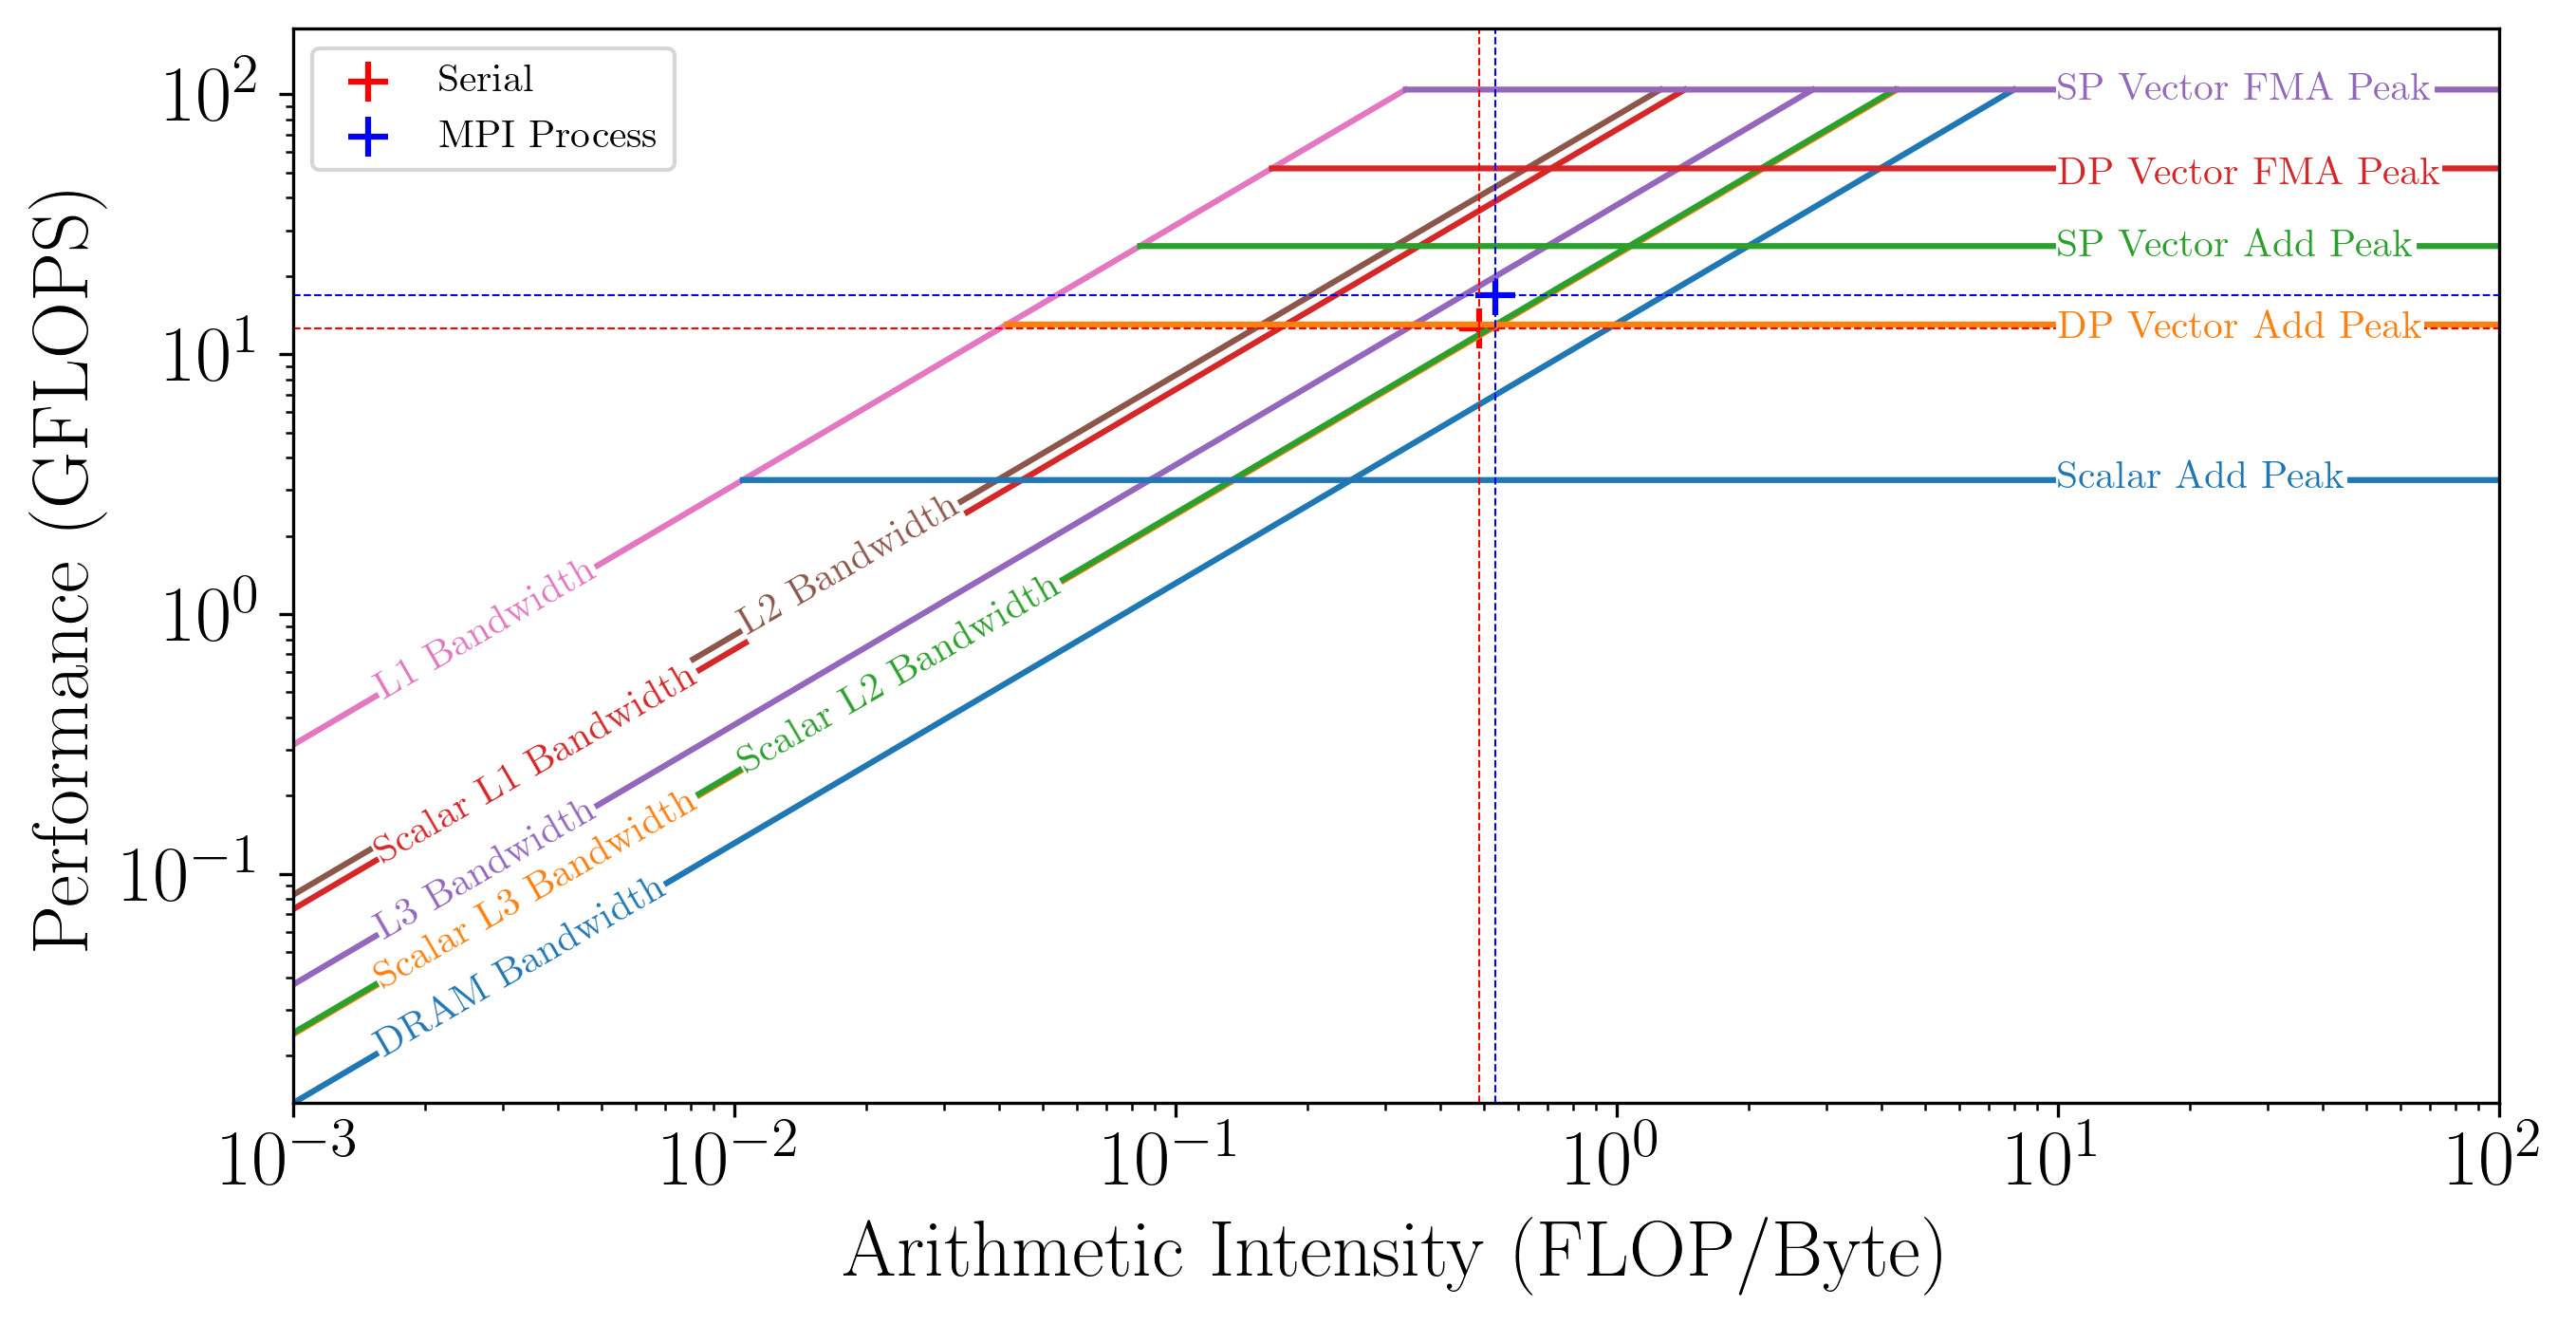
\includegraphics[width=\linewidth]{roofline.png}
  \caption{Roofline model of the \texttt{timestep} loop run on the $1024\times1024$ test case}\label{fig:roofline}
\end{figure}

On the $1024 \times 1024$ test case, each process in my MPI implementation achieved an arithmetic intensity of 0.533 FLOP/Byte and 16.905 FLOP/s of performance during the \texttt{timestep} procedure.
Compared to my serial implementation, the arithmetic intensity was approximately identical, which was expected since I made very few changes to the procedure.
However, the performance increased by 35\% because the program did not have to interact with the DRAM, which had a lower bandwidth, as often.
For example, in the \texttt{timestep} procedure in my MPI implementation, less than 0.01 GB of data was passed through DRAM.
In comparison, in my serial implementation, 2306.03 GB of data was passed through the DRAM.

My MPI implementation had a large overhead introduced by the \texttt{halo\_exchange} procedure.
In fact, when ran with 112 ranks on the $1024\times1024$ test case, 23\% of the compute time of my program was spent in this procedure.

\section{Hybrid MPI and OpenMP}

I sought to investigate whether a hybrid implementation that used both MPI and OpenMP would execute faster than my prior implementation.

\subsection{OpenMP vs MPI Scaling}

Before producing my hybrid implementation, I compared the speedup curves of my MPI implementation to those of my OpenMP implementation.
Figure \ref{fig:scaling_openmp_mpi} displays the speedup curves of these two implementations for the $128 \times 128$ and the $1024 \times 1024$ grid sizes.

\begin{figure}[htpb]
  \centering
  \resizebox{\columnwidth}{!}{
    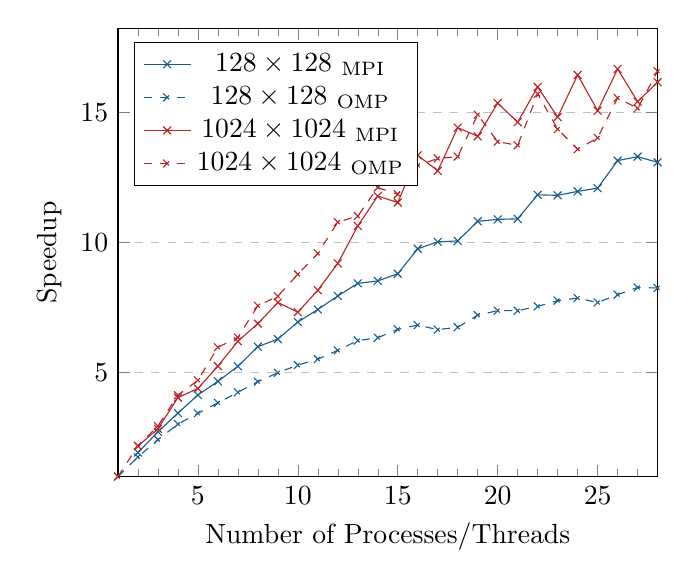
\begin{tikzpicture}
      \begin{axis}[
        xlabel={Number of Processes/Threads},
        ylabel={Speedup},
        xmin = 1, xmax = 28,
        ymin = 1,
        % xtick={0, 5, 10, 15, 20, 25},
        % ytick={0,20,40,60,80,100,120},
        legend pos=north west,
        ymajorgrids=true,
        grid style=dashed,
        minor xtick = {1, 2, 3, 4, 5, 6, 7, 8, 9, 10, 11, 12, 13, 14, 15, 16, 17, 18, 19, 20, 21, 22, 23, 24, 25, 26, 27, 28}
      ]
      \addlegendentry{$128\times128$ \textsubscript{MPI}}
      \addplot[color = {rgb:red,31;green,119;blue,180}, mark = x]coordinates{
        (1)
        (2, 1.923484904)
        (3, 2.720894881)
        (4, 3.440629879)
        (5, 4.138267014)
        (6, 4.663357796)
        (7, 5.242110909)
        (8, 5.997834661)
        (9, 6.289791841)
        (10, 6.946565607)
        (11, 7.428037519)
        (12, 7.95038628)
        (13, 8.433876381)
        (14, 8.529248058)
        (15, 8.803834029)
        (16, 9.766209845)
        (17, 10.03121078)
        (18, 10.06840901)
        (19, 10.823501)
        (20, 10.89601518)
        (21, 10.91800443)
        (22, 11.84262736)
        (23, 11.8219416)
        (24, 11.97369741)
        (25, 12.0975617)
        (26, 13.1584053)
        (27, 13.31030358)
        (28, 13.09199604)
      };
      \addlegendentry{$128\times128$ \textsubscript{OMP}}
      \addplot[color = {rgb:red,31;green,119;blue,180}, mark = x, dashed]coordinates{
        (1, 1.0)
        (2, 1.7525169788462858)
        (3, 2.419897249840069)
        (4, 3.0177321760395954)
        (5, 3.4340474353625594)
        (6, 3.8362657949346852)
        (7, 4.241072726461517)
        (8, 4.651864978037027)
        (9, 4.993654422331282)
        (10,5.2882280154084835)
        (11,5.520195387872089)
        (12,5.854579031493787)
        (13,6.23457059163917)
        (14,6.342501046595846)
        (15,6.666023078680611)
        (16,6.829810732132427)
        (17,6.6526516481296065)
        (18,6.746204776109836)
        (19,7.213003419569139)
        (20,7.383978810814603)
        (21,7.383266518002555)
        (22,7.548589923892521)
        (23,7.770076587082373)
        (24,7.86829502746941)
        (25,7.69660960948019)
        (26,8.000150678051229)
        (27,8.274732001825265)
        (28,8.256913368882064)
      };
      \addlegendentry{$1024\times1024$ \textsubscript{MPI}}
      \addplot[color = {rgb:red,214;green,39;blue,40}, mark = x]coordinates{
        (1)
        (2, 2.173711193)
        (3, 2.836895868)
        (4, 4.036873172)
        (5, 4.389001279)
        (6, 5.250171877)
        (7, 6.206328606)
        (8, 6.884988543)
        (9, 7.699455735)
        (10, 7.326102008)
        (11, 8.167957305)
        (12, 9.202796572)
        (13, 10.64605845)
        (14, 11.79316736)
        (15, 11.54612272)
        (16, 13.36192713)
        (17, 12.76637316)
        (18, 14.4268392)
        (19, 14.09500759)
        (20, 15.37438851)
        (21, 14.63591628)
        (22, 15.99456741)
        (23, 14.83351358)
        (24, 16.4555638)
        (25, 15.07849263)
        (26, 16.68441375)
        (27, 15.42876319)
        (28, 16.17670295)
      };
      \addlegendentry{$1024\times1024$ \textsubscript{OMP}}
      \addplot[color = {rgb:red,214;green,39;blue,40}, mark = x, dashed]coordinates{
        (1, 1)
        (2, 2.182054561)
        (3, 2.943754524)
        (4, 4.131667716)
        (5, 4.705750019)
        (6, 5.973656817)
        (7, 6.351981192)
        (8, 7.573833461)
        (9, 7.941396106)
        (10,8.7813412)
        (11,9.58468842)
        (12,10.78916878)
        (13,11.02458512)
        (14,12.12324785)
        (15,11.86351157)
        (16,12.97218687)
        (17,13.23885542)
        (18,13.31481491)
        (19,14.92644603)
        (20,13.88484436)
        (21,13.74639988)
        (22,15.72695273)
        (23,14.36825215)
        (24,13.59839996)
        (25,14.03417467)
        (26,15.5747082)
        (27,15.16956075)
        (28,16.59876059)
      };
      \end{axis}
    \end{tikzpicture}
  }
  \caption{Speedup curves for my OpenMP and MPI implementation}\label{fig:scaling_openmp_mpi}
\end{figure}

My MPI implementation scaled better for the smaller grid, whereas my OpenMP implementation initially scaled slightly better for the larger grid.
This was because each implementation had a different overhead: in the OpenMP implementation, the overhead arose from the creation and synchronisation of threads each timestep; in the MPI implementation, the overhead arose from the halo exchange.
The OpenMP overhead was largely constant regardless of the grid size, whereas the MPI overhead was correlated with the width of the grid.

\subsection{Implementation}

Having gained an understanding of how my OpenMP and MPI implementations scaled, I hypothesised that a hybrid implementations would reduce the execution times for large, wide grid sizes.
Therefore, I produced three additional grids to test my implementation with.

Using my prior implementation as a starting point, I replaced the call to the \texttt{MPI\_Init} procedure with a call to the \texttt{MPI\_Init\_thread} procedure, passing \texttt{MPI\_THREAD\_FUNNELED} as the third argument since only the main thread was to make MPI calls.
I parallelised the outer loop in the \texttt{timestep} procedure with OpenMP, and set the \texttt{I\_MPI\_PIN\_DOMAIN} environment variable to \texttt{socket}.

I tested my implementation with eight processes---one per socket across four nodes---communicating via MPI, with each process creating fourteen threads.
Table \ref{tab:hybrid} displays the results of my experiment.
As anticipated, the hybrid implementation was slower with the smaller grids that were provided, but faster with the larger grids that I produced myself.

\begin{table}[htbp]
  \begin{center}
  \caption{Execution times with the hybrid implementation and speedup over the prior implementation}\label{tab:hybrid}
  \begin{tabular}[t]{l | l l} 
      \hline\hline
      Grid Size&Time (s)&Speedup\\
      \hline
      $128 \times 128$&\texttt{ \space0.67}&\texttt{}\\
      $128 \times 256$&\texttt{ \space0.73}&\texttt{}\\
      $256 \times 256$&\texttt{ \space1.94}&\texttt{}\\
      $1024 \times 1024$&\texttt{ \space3.17}&\texttt{}\\
      \hdashline
      $4096 \times 1024$&\texttt{ 15.99}&\texttt{1.42}\\
      $8192 \times 1024$&\texttt{ 53.88}&\texttt{1.03}\\
      $16384 \times 1024$&\texttt{102.34}&\texttt{1.15}\\
      \hline
    \end{tabular}
  \end{center}
\end{table}

\section{GPU Programming}

GPUs typically have 3--5x the memory bandwidth, and 5--10x the peak FLOP/s that CPUs have.
This is true for BC4, in which a single NVIDIA Tesla P100 has 4.8x the peak memory bandwidth, and 9.8x the peak double precision performance that two Intel E5-2840 v4 CPUs have \cite{youtube}.
OpenCL is a framework for heterogeneous computing that can be used for GPU programming.
I sought to produce an implementation of LBM built with OpenCL.

\subsection{Implementation}

I used my serial optimised implementation as a starting point for my host program.
To ensure my program was portable, I used the \texttt{clGetPlatformIDs} and \texttt{clGetDeviceIDs} procedures to produce an array of all devices available to the host program, and selected the device defined by the \texttt{OCL\_DEVICE} environment variable.
For the selected device, I created a single context and a single in-order queue.
I opted to keep my \texttt{cells} and \texttt{cells\_new} data in the SoA format, since coalesced memory accesses are key for high bandwidth.

I converted the \texttt{accelerate\_flow} and \texttt{timestep} procedures into kernels to run on the GPU.
Transerring memory between host and device is a slow operation; therefore, I opted to store the partial average velocities of each timestep in global memory on the device.
Each timestep, the \texttt{timestep} kernel performed a parallel reduction to sum the velocities of each cell in the same work group.
I opted to implement a parallel reduction to minimise the number of addition operations.
I summed the average velocities of each work group on the host device once all iterations had been complete.

Table \ref{tab:OpenCL} displays execution times of my OpenCL implementation ran on a single NVIDIA Tesla P100.
I also calculated the speedup over my implementation built with distributed memory parallelism across four nodes of BC4.
My OpenCL implementation was slower for the four grid sizes provided, but faster for the two grids I produced myself.

\begin{table}[htbp]
  \begin{center}
  \caption{Execution times with the OpenCL implementation and speedup over the serial implementation}\label{tab:OpenCL}
  \begin{tabular}[t]{l | l l} 
      \hline\hline
      Grid Size&Time (s)&Speedup\\
      \hline
      $128 \times 128$&\texttt{}&\texttt{}\\
      $128 \times 256$&\texttt{}&\texttt{}\\
      $256 \times 256$&\texttt{}&\texttt{}\\
      $1024 \times 1024$&\texttt{}&\texttt{}\\
      \hdashline
      $2048 \times 2048$&\texttt{}&\texttt{}\\
      $4096 \times 4096$&\texttt{}&\texttt{}\\
      \hline
    \end{tabular}
  \end{center}
\end{table}

\subsection{Work-Group Size}

The size of the work-group has significant implications on performance.


I previously used a local size of 16 cells in the $y$ direction, and 32 cells in the $x$ direction.


\section{Conclusion}

In conclusion, all three of the implementations I produced and tested significantly improved the performance of \texttt{d2q9-bgk.c}.

\printbibliography

\end{document}